\FrontmatterChapter{Abstract}
{\setlength{\parindent}{0pt}
\begin{Large}
\textbf{OPTIMIZATION OF AN ARTIFICIAL VISION SYSTEM OF AN INDUSTRIAL ROBOT FOR A PICK AND PLACE APPLICATION}
\end{Large}

\textbf{Author: Ortiz de Zúñiga Mingot, Ignacio.} \\
Supervisors: Boal Martín-Larrauri, Jaime y Rodríguez Mondéjar, José Antonio. \\
Collaborating Entity: ICAI – Universidad Pontificia Comillas \\

\section*{Abstract}
In the last decade an industrial revolution known as industry 4.0 has started. This change has been capable thanks to the development and growth of industrial robots. This robots are now capable of completing task previously impossible to humans and at a faster and more efficient rate. Because of this advances Comillas ICAI has decided to implant this new systems to it's industrial robots. This robots have to be capable of identifying and recollecting LEGO pieces randomly set at a work bench. To do so this project takes upon the previous work of Ana Berjón Valles to improve it. It will also create new systems base on convolutional neuronal networks and R-CNN, Faster R-CNN and YOLO.
\textbf{Keywords:} Artificial vision, Neuronal networks, AlexNet, VGG-16, R-CNN, Faster R-CNN, YOLO, Robotics, LEGO

\section*{1. Introduction}
In the past two years Comillas ICAI has been developing a system capable of endowing artificial vision and autonomy to it's robots. This robots have to be capable of identifying and recollecting LEGO pieces randomly set at a work bench. This project takes upon this previous work done by Ana Berjón Valles to improve it. To do so, we have first upgraded the current segmentation system base on colour masking, edge detection and the Hough transform. Also the systems designed to analyse the depth and rotation of the pieces has been redesigned and upgraded. However, despite this upgrades our system is still incapable to compete with the modern systems already well implanted in the industry. This new systems are based on convolutional neuronal networks. As it's name indicates this networks are based on the principles of convolution and deep learning. Because of it we have decided to upgrade the robots with this new technologies and improve it's capabilities.

\section*{2. Methodology}
The current artificial vision system implanted on the robot is composed by three elements that must cooperate and communicate with each other. The communications are done via USB and TCP/IP. The capture of images is done by the camera Intel Realsense D435. This camera contains RGB and Depth sensors and it is connected to the system with and USB connexion. The processing of both RGB and Depth images is done by a computer with the help of MATLAB. And lastly, the instructions containing the position, height and orientation of the pieces is send to the IRB120 robot with a TCP/IP connection. The architecture of the system can be seen on \autoref{fig:abs1}.

\begin{figure}[ht]
	\centering
	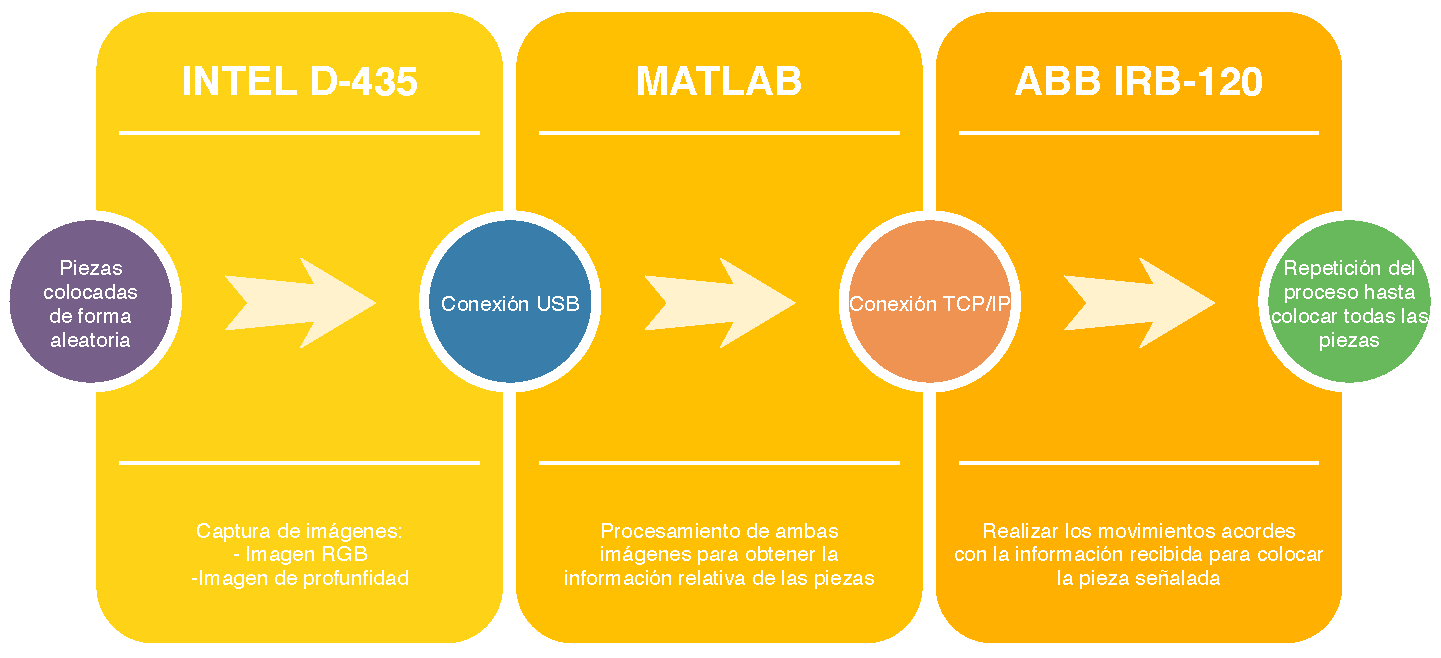
\includegraphics[width=0.9\textwidth]{Introduccion/Esquema_arquitectura.pdf}
	\caption{Architecture of the system}
	\label{fig:abs1}
	\vspace{-5pt}
\end{figure}

The first step on the development of this project is to upgrade the current system based on colour masking, edge detection and the Hough transform. The colour filters have been revised and upgraded to reduce the number of false positives and the analysis based on edge detection has been perfected. The communication with the camera has been redone to allow for a faster capture and to eliminate the distortion of the depth image. The analysis and calculation of the orientation of each pieces has been redone and upgraded with a new an more sophisticated analysis method also based on the Hough transform. 

Once the current system has been upgraded and perfected, new object detectors based on convolutional neuronal networks have been develop from zero. In order to create a rigorous comparison between different neuronal networks multiple networks have been created. To evaluate different technologies we have created networks of the type R-CNN, Faster R-CNN and YOLO. Also to be able to evaluate the impact of the size of the network ours are based on two different classifiers. The selected classifiers are a retrained version of AlexNet and VGG-16. The retraining of these classifiers has also been done by us.

The use of classifiers as the base for an object detector is because it reduces the training time while also improving the results of the network. This process is known as transfer learning and is common step use on the creation of object detectors. That's the reason why we have decided to use AlexNet ang VGG-16. We have decided to use these network so that we could evaluate the impact of different networks size and to demonstrate the evolution of neuronal networks. AlexNet was created on 2012 while VGG-16 is from 2014 and currently is still a very modern and capable network. But because this networks where never created to identify LEGO pieces we had to first retrain them so that they could learn the characteristics of LEGOs. These new classifiers have been renamed LEGONet and LEGO16 respectively and will be used as the base for our object detectors. Two networks type R-CNN, two type Faster R-CNN and two type YOLO.

R-CNN emerged as the evolution of first object detectors based on Sliding windows. This networks firstly analyses the image and proposes approximately 2000 regions of interest to be analyse. Then a classifier analyses each of the regions independently to determine the existence of an object inside the regions. With this system the execution time was improve compared to the Sliding windows systems but it still is a slow process compared to newer systems. In exchange for it's poor performance this system is characterize for having good precision. During the development of this project two networks base on LEGONet and LEGO16 have been created. This networks type R-CNN have been trained with a dataset created by us and multiple testing has been conducted to determine the best training options.

Faster R-CNN was created three years after R-CNN and emerges as an evolution of this system. As R-CNN this new system is also based on regions proposal but this task is done by a RPN network. RPN is a convolutional neuronal network whose output are the proposed regions to analyse. The RPN network is located after the first convolutional networks and takes information from them and then the rest of the network analyses the regions proposed by the RPN. In this system the original image is not analyse as many times as regions proposed instead is the output from the convolutional layers that is analyse multiple times. Thanks to this the system has a better performance than R-CNN and it manages to reduce training and executing times. During the development of this project two networks type Faster R-CNN base on LEGONet and LEGO16 have been created. This networks have been trained with a dataset created by us and multiple testing has been conducted to determine the best training options.

YOLO is one of the newest and modern systems for object detection. It is characterize for it's performance and speed both in training and execution. This is because as it's name indicates, You Only Look Once, it only analyses the image one time. And system designed to predict the bounding boxes predicts them. Compare to the previously mentioned systems, YOLo is characterize for it's ability to see the whole image. This allows it to create connexions between different elements of the image and it helps it to reduce the number of false positives. During the development of this project two networks type YOLO base on LEGONet and LEGO16 have been created. This networks have been trained with a dataset created by us and multiple testing has been conducted to determine the best training options.

Once the pieces have been identified with the use of the object detector it's time to calculate their orientation and height. This process has already been perfected at the beginning of the project. The information extracted from all this systems is then process and send to the robot to relocate the pieces.

As an additional development of the project we have decided to create to regression models based on LEGONet and LEGO16 to estimate the orientation of each LEGO piece. For the development of this networks a new dataset has been created by us composed by thousand of images of LEGOs rotated with different angles. For the training of the networks multiple testing has been done to determine the best training options.

\section*{3. Results}
\subsection*{Object detectors}
A comparative of all the object detectors has been done. This includes the classic system based of colour masking, edge detection and th Hough transform. The evaluation has been done by analyzing a total of 380 LEGO pieces of different colours and in different scenes. With these evaluation multiple measures have been taken to evaluate the behaviour of each object detector.

\subsubsection*{Precision, Recall, Failure rate and FPPI}
As mentioned before, multiple measures have been taken from different parameters to evaluate the behaviour of each system. The precision indicates the level of similarity between the region proposed by the detector and true region of the piece. The recall determines the relationship between the number of true positives and the number of false negatives. The failure rate indicates the probability of not detecting a piece on an image. And the FPPI represents the number of False Positives Per Image detected. Analyzing the results of all the object detectors on the evaluation we can observe the clear superiority of neuronal networks. The new detectors are capable of detecting the pieces under different illumination and scenes. While also reducing the number of false positives and the failure rate. 

\begin{figure}[ht]  %Estudio Azul
\vspace{-10pt}
  \subfloat{
	\begin{minipage}[c][1\width]{0.49\textwidth}
	   \centering
	   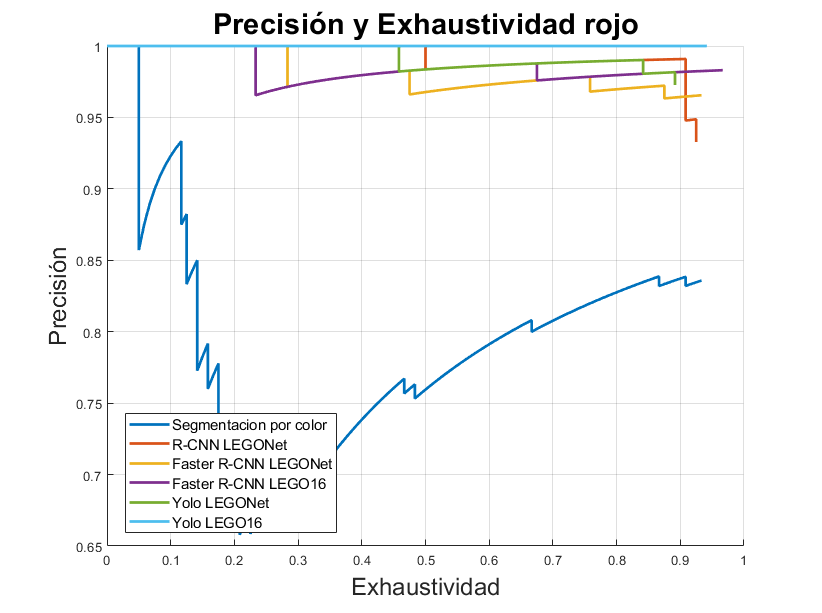
\includegraphics[width=1\textwidth]{Resultados/precision red.png}
	\end{minipage}}
  \hfill	
  \subfloat{
	\begin{minipage}[c][1\width]{0.49\textwidth}
	   \centering
	   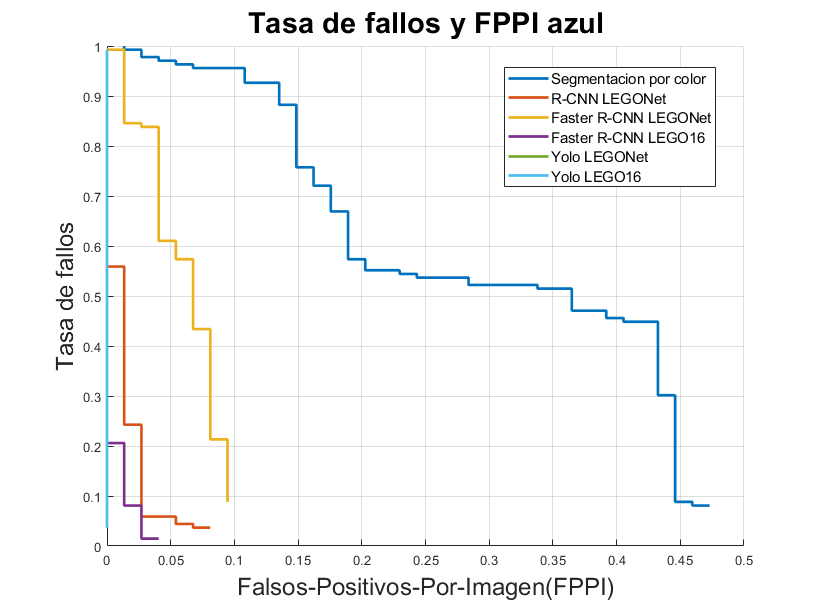
\includegraphics[width=1\textwidth]{Resultados/miss blue.png}
	\end{minipage}}
\caption{Comparison of the different segmentation methods to detect red LEGO pieces}
\label{fig:abs2}
\end{figure}

\subsubsection*{Speed}
Another important factor to consider when analyzing all the object detectors is the execution time. Because of it we have measure the time taken by each detector to analyse all the images from the evaluation. This measures on tenths of a second have been transform to images per second to help understand the capabilities of each detector. We can see that all the new systems are faster than the previous classical system. With the exception of R-CNN whose performance is similar to the classical system. The networks taht stand out the most are the ones based on YOLO. Their performance is clearly superior always achieving to break the 30 fps barrier and in the case of YOLo based on LEGONet also the 60 fps barrier.

\begin{figure}[ht]  %Cajas velocidad
\vspace{-10pt}
	\centering
	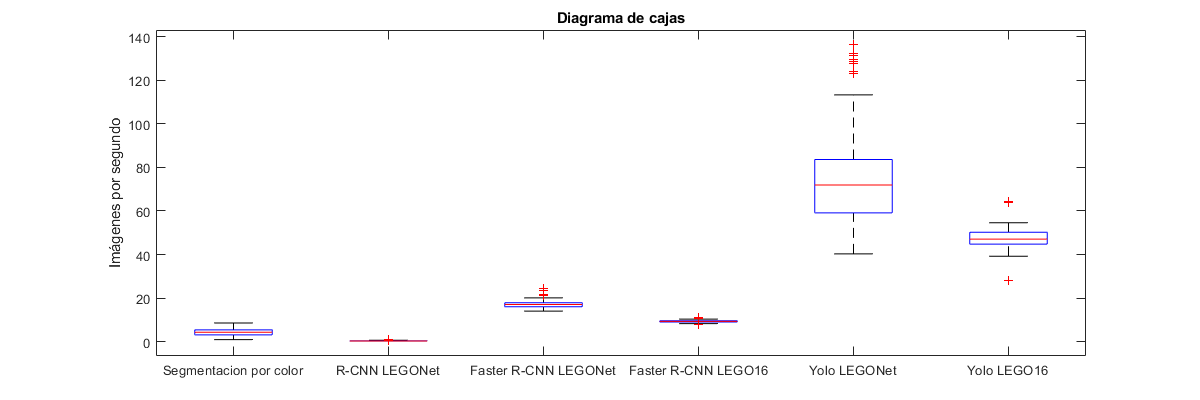
\includegraphics[width=1\textwidth]{Resultados/detectores cajas.png}
	\caption{Box diagrams: comparison of the speed of different object detectors (Higher is better)}
	\label{fig:abs3}
\end{figure}

\subsection*{Analysis of the orientation}
An evaluation of the methods designed to calculate the orientation of each piece has also been done. We have compare all three systems. The classical system based on edge detection and the Hough transform and the two networks based on LEGONet and LEGO16. The evaluation has measured different parameters of these systems. The mean error, the maximum error, the typical deviation and the speed of each method. In this evaluation the execution time of each system has also been transform into pieces per second to help understand the capabilities of each method.

\begin{table}[ht] %tabla orientación precision
  \centering
    \begin{tabular}{|l|r|r|r|}
    \cline{2-4} \multicolumn{1}{r|}{} & \multicolumn{1}{l|}{Hough transform} & \multicolumn{1}{l|}{LEGONet} & \multicolumn{1}{l|}{LEGO16}\\	
    \hline
    Mean error & 0.98$^{\circ}$  & 0.33$^{\circ}$ & 0.71$^{\circ}$ \\
    \hline
    Maximum error & 26$^{\circ}$  & 1.3$^{\circ}$ & 16$^{\circ}$ \\
    \hline
    Precision & 83.67\% & 97.67\% & 79.33\% \\
    \hline
    Typical deviation & 1.82$^{\circ}$ & 0.43$^{\circ}$ & 1.23$^{\circ}$ \\
    \hline
    Pieces per second	&	89.7	&	74.6	&	178.5	\\
    \hline
    \end{tabular}%
  \label{tab:abs4}%
  \caption{Comparative of the mean error, the maximum error, precision, the typical deviation and speed of each method for calculating the orientation of pieces}
\end{table}

\begin{figure}[ht]  %Cajas orientación precision
	\centering
	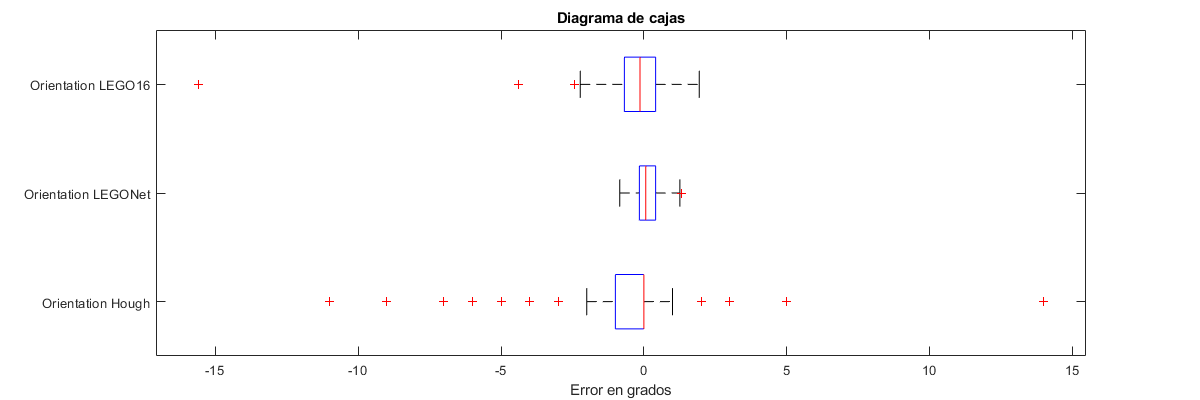
\includegraphics[width=0.95\textwidth]{Resultados/orientacion precision cajas.png}
	\caption{Box diagram: Comparison of the precision of different methods for calculating the orientation of pieces (the closer to the zero the better)}
	\label{fig:abs5}
\end{figure}

\section*{4. Conclusions}
The objective of this project is the perfection of a previous system developed by Ana Berjón Valles \citep{TFGAna}. All the objectives set during the development of this project have been successfully completed. Bellow we will develop in more detail all these objectives.

One of the principal task was to subsidize the problems of the old system with the changes of illumination. The classic system is based on colour filtering and because of it a change on the illumination could easily affect it's capacity to detect a piece. The new systems based on neuronal networks are more robust and their performance does not variate as much with changes in illumination. More testing needs to be done to evaluate this results on the laboratory but considering the results of the evaluation we consider that this problem has been solved and mitigated. Considering the results we recommend to future projects to implement a system with YOLO based on LEGO16 and the regression model based on LEGONet. Or a combination of multiple neuronal networks.

Another limitation of the previous system was the failures due to a bad analysis of the depth image. Due to the type of technology used to obtain the depth image, the camera is really sensible to reflexes. This problem has been solved with the modification of the analysis of depth. The work bench is divided of sections and the height of each section is estimated with a median. Thanks to the inclusion of these steps and the capability to recalibrate de system we have mitigated the effect of the reflexes

Generalization of the algorithms. During the development of this project we have consider the possibility to implement these system for different applications or robots. Because of it the process of both RGB and Depth images doesn't depend of the camera, the position or the robot. The analyse of the depth image can be easily calibrated to work under different circumstances and positions with the help of the calibration function created. The images process can also be retrain to detect different pieces. And all the processed related with the robot has been done separate from the image processing so it can easily modify to be use on another robot.

Globally analyzing the project we can conclude that the new systems suppose a bid upgrade compare to the previous systems. Once it is implanted it will suppose a big upgrade on the technologies and capabilities of the industrial robot of Comillas ICAI.
}